% ---------------------------------------------------------------------
% Das Dokument kompiliert mit pdflatex und ist auf Basis
% von Koma-Script entstanden.
%
% Autor des Templates (für Anmerkungen):
% Michael von Riegen, riegen@informatik.uni-hamburg.de
%
% Einzelne Code-Teile für das Titelblatt sind aus dem Template
% von Benjamin Kirchheim entnommen.
%
% 25.05.09, Frank Langanke: Vorlage auf aktuelle KOMA-Version aktualisiert
% 26.05.09, Michael von Riegen: Anmerkung --> aktuelles Koma-Script ist nötig!
% 17.10.2016 Version ohne Logo
% ---------------------------------------------------------------------
\documentclass[11pt,DIV=15,BCOR=20mm,bibliography=totoc]{scrbook}

% Import von Paketen und Optionen die das gesamte Dokument betreffen
% sind in myPreamble.sty ausgelagert.
\usepackage{preamble}

% Arbeitet man nur an einem Kapitel, wird durch folgenden Befehl nur dieses eingebunden.
% Spart manuelles auskommentieren von vielen include-Befehlen;
% hat keine Auswirkung auf input-Befehle
% \includeonly{kapitel1}

\begin{document}

% TITELSEITE
\begin{titlepage}

	% Fehler "destination with the same identifier" unterdrücken...
  \setcounter{page}{-1}

	% Titelseite
	\begin{figure}[h]
		UNIVERSITÄT HAMBURG\\
FAKULTÄT FÜR MATHEMATIK, INFORMATIK \\
UND NATURWISSENSCHAFTEN

		\vspace{1cm}
	\end{figure}

	\vfill
	
	\begin{center}
		% Diplomarbeit 
		\noindent { \huge
			Bachelorarbeit \\
		}
		\vspace{14mm}
		% Titel
		\noindent \textbf{\huge
		  Eine Vorlage für studentische Arbeiten \\im Arbeitsbereich VSIS \\
		}
		\vspace{60mm}	
	\end{center}
	
	\vfill
	
	\noindent \textbf{Max Peter Mustermann} \\
	\noindent \rule{\textwidth}{0.4mm} 
	\noindent{\textrm{max.peter.mustermann@informatik.uni-hamburg.de}} \\
	\noindent{\textrm{Studiengang Informatik}} \\
	\noindent{\textrm{Matr.-Nr. 12345678}} \\
	\noindent{\textrm{Fachsemester 99}} \\
	\begin{tabbing}
	\hspace{8em} \=  \kill
	Erstgutachter: \> Professor A. Ersthelfer \\
	Zweitgutachter: \> Professor Z. Eswirdschonwerden \\
	~ \\
	Abgabe: 09.2017
	\end{tabbing}
	
	% Rückseite der Titelseite mit Zitat
	\newpage 
	\thispagestyle{empty}
	\setcounter{page}{0}

	% wenn man Lust auf ein Zitat hat...
	% ... ansonsten auskommentieren
	~\\ \vfill \noindent 
	A distributed system is one where the failure of some \\
	computer I've never heard of can keep me from getting my work done. \\
	\textit{-- Leslie Lamport}
\end{titlepage}



% VERZEICHNISSE (Inhaltsverzeichnis, Abkürzungen)
% Vorspann einleiten --> Seitennummerierung römisch
\frontmatter

% Inhaltsverzeichnis

\begingroup
\let\cleardoublepage\clearpage
\tableofcontents
% \listoffigures
% \listoftables
\endgroup

% Hauptteil einleiten --> Seitennummerierung wieder arabisch
\mainmatter

\chapter{Einleitung}

Vor einiger Zeit wurde Software primär mit dem Hintergrund entwickelt später auf einem einzelnen Rechner zu laufen, sodass man nicht mit vielen Seiteneffekten durch eine andere Konfiguration auf Software- oder Hardware-Ebene zu rechnen hatte. Heute arbeiten viele Entwickler gleichzeitig auf verschiedensten Geräten an einer einzelnen Webanwendung oder einem Webservice. Es gibt eine unendliche Anzahl von Konfigurationen durch verschiedene Hardware-Konfigurationen, verschiedene Betriebssysteme oder Versionen oder auch installierte Programme und Dienste. All diese Unterschiede können die entwickelte Anwendung bereits im Entwicklungsstadium auf unterschiedliche Weise beeinflussen und für unterschiedliches Verhalten sorgen. Wird die Anwendung später ausgerollt und auf einem Server ausgerollt, muss sie wiederum in einer anderen Umgebung arbeiten. Das Ziel ist es deswegen die Software nicht von der Plattform auf der sie ausgeführt wird abhängig zu machen und sie immer in der gleichen Umgebung laufen zu lassen. Damit kann die Software auf beliebig vielen System ausgeführt werden mit gleichzeitiger Sicherheit, dass sie sich auf allen Systemen gleich verhalten wird. Um dies zu ermöglichen kann die Software entweder in einer virtuellen Maschine, einem simulierten Rechner, oder einem Container, einer leichtgewichtigeren Form der Virtualisierung, ausgeführt werden. Im Folgenden werde ich auf die Arbeitsweise von Containern im Vergleich zu virtuellen Maschinen eingehen und im speziellen Docker, einer Software für eine einfachere Handhabung von Containern, vorstellen.

\chapter{Grundlagen}

% -----------
% --- VMs ---
% -----------

\section{Virtuelle Maschinen}
Als virtuelle Maschine (kurz VM) wird in der Informatik die Nachbildung eines Rechnersystems bezeichnet. Die virtuelle Maschine bildet die Rechnerarchitektur eines real in Hardware existierenden oder hypothetischen Rechners nach \cite{Sieg2007}. Den virtuellen Maschinen wird über den sogenannten Hypervisor oder auch Virtual Machine Monitor (VMM) ein komplettes System vorgespielt, sodass diese die zugeteilten Ressourcen für echte Hardware halten \cite{OSTEP}.\\

\begin{figure}[!ht] % see https://en.wikibooks.org/wiki/LaTeX/Floats,_Figures_and_Captions for placement parameters
  \centering
  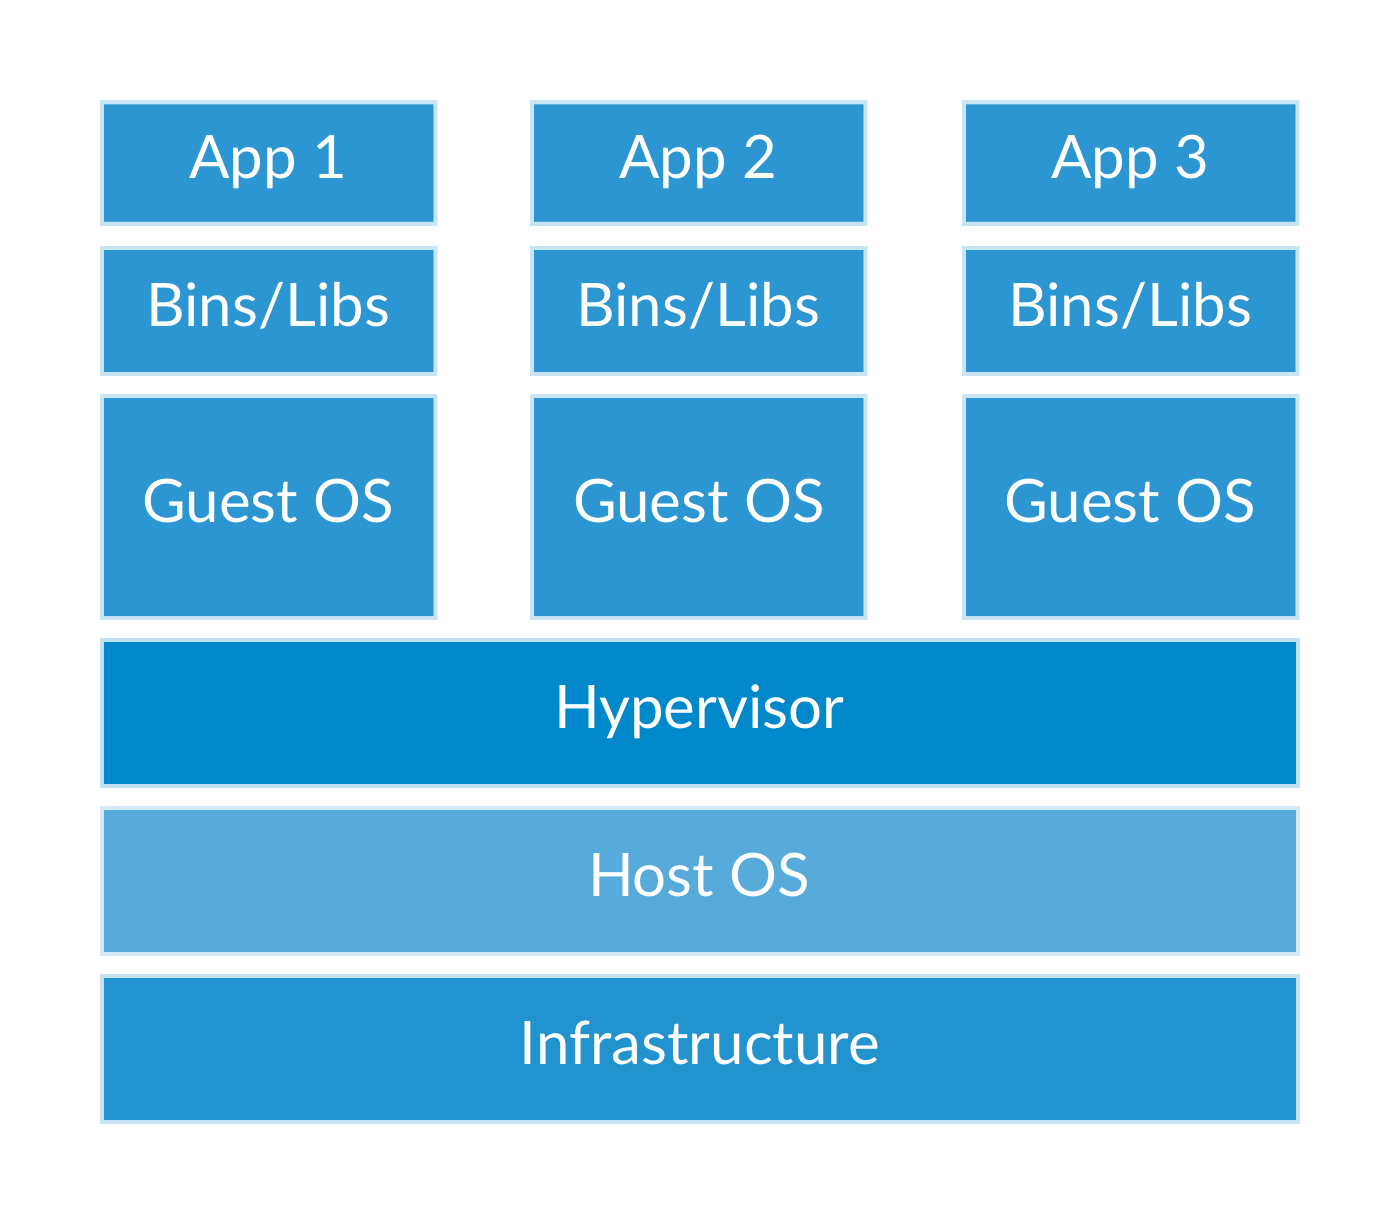
\includegraphics[width=0.5\textwidth]{images/1-docker-vm.png}
  \caption{Mehrere virtuelle Maschinen auf einem Host-System. \cite{docker}}
\end{figure}

\noindent Da neben der Applikation selbst noch eine ganze Reihe weiterer Ressourcen benötigt werden, nämlich das Betriebssystem und Bibliotheken führt dies zu höherem Ressourcenverbrauch und großen Abhängigkeiten vom Betriebssystem.\linebreak Zum Beispiel können bei einem Update des Betriebssystems für die Applikation nötige Bibliotheken verändert werden, die ein verändertes Verhalten hervorrufen. Dies bedeutet sowohl einen hohen Overhead an verbrauchten Systemressourcen, als auch einen hohen Wartungsaufwand.\\

\noindent Es wird meist zwischen Typ-1-Hypervisor und Typ-2-Hypervisor unterschieden. Inzwischen ließt man auch öfter von einem Typ-0-Hypervisor, einer neueren Technologie, auf die ich in dieser Arbeit nicht weiter eingehen werde.\\

\noindent Ein Typ-1-Hypervisor (native oder bare-metal) setzt direkt auf der Hardware auf und benötigt keine vorherige Betriebssystem-Installation, muss aber von der entsprechenden Hardware unterstützt werden.

\vspace{\baselineskip}

\noindent Ein Typ-2-Hypervisor (hosted) setzt auf einem vollwertigen Betriebssystem auf und nutzt die Gerätetreiber des Betriebssystems, um auf die Hardware des Hostsystems zuzugreifen. \cite{wiki:hyper}, \cite{6903537}\\

\begin{figure}[!ht] % see https://en.wikibooks.org/wiki/LaTeX/Floats,_Figures_and_Captions for placement parameters
  \centering
  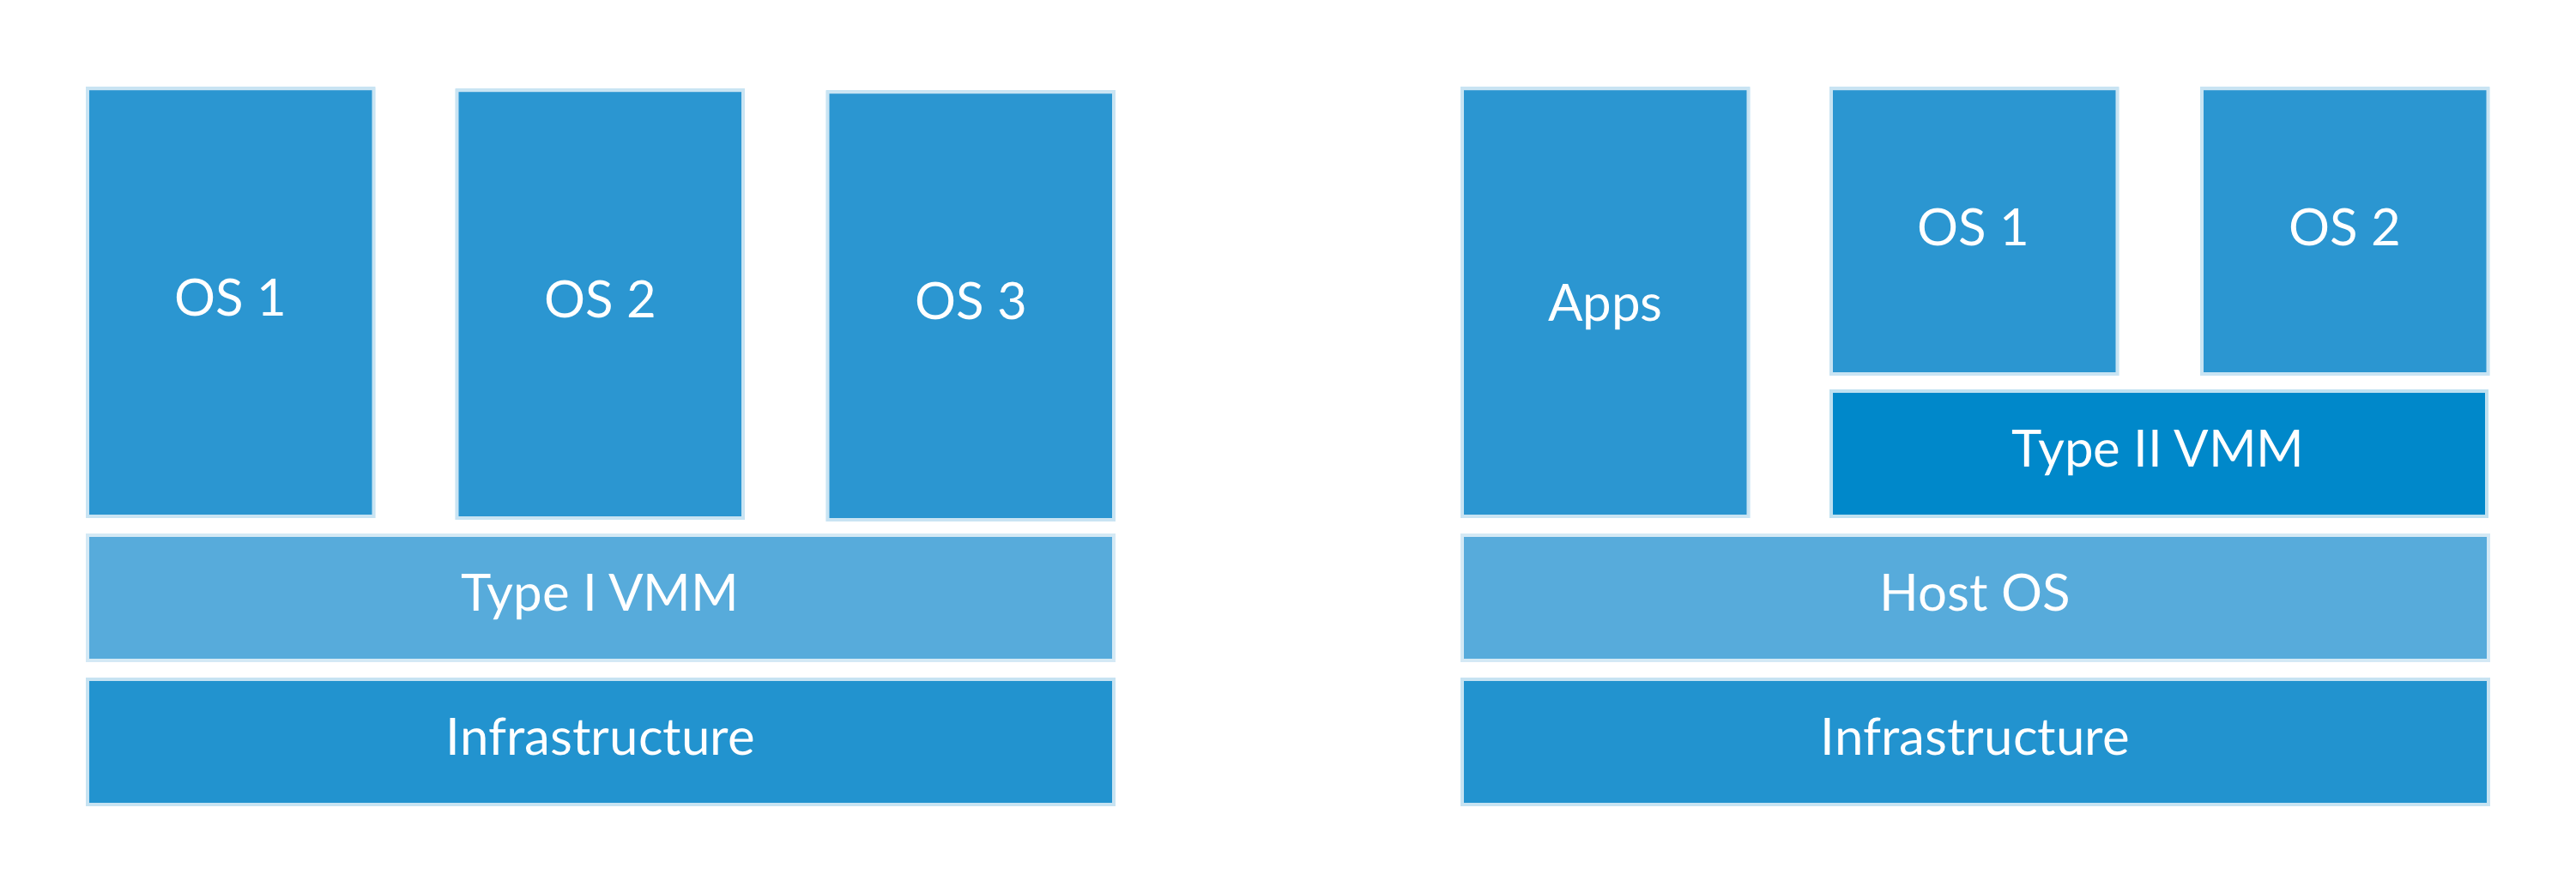
\includegraphics[width=1\textwidth]{images/2-hypervisors.png}
  \caption{Typ-1-Hypervisor und Typ-2-Hypervisor. \cite{wiki:hyper}}
\end{figure}

% ---------
% Container
% ---------

\section{Container}
Ein Gegenentwurf zu virtuellen Maschinen sind sogenannte Container, die das Ziel haben, mit weniger Overhead den gleichen Grad an Isolation und Sicherheit zu liefern.

\paragraph{}
\noindent Anders als virtuelle Maschinen, teilen sich Container das Betriebssystem bzw. den Kernel mit dem Hostsystem auf dem die Container gestartet werden. Befehle können also nahezu direkt auf der Hardware ausgeführt werden und müssen nicht erst, wie bei virtuellen Maschinen den Umweg über den Hypervisor gehen, was einen offensichtlichen Performancevorteil mit sich bringt, schränkt die Container aber auch dahingehend ein, dass nur Anwendungen mit dem gleichen Kernel wie dem des Hosts gestartet werden können. So können also zum Beispiel nicht nativ Windows Container in einer Linux-Umgebung gestartet werden und umgekehrt \cite{7092949}. Wie auch virtuelle Maschinen werden Container auf Basis von Images erstellt. Diese Container können gestoppt und gestartet werden.\\ Es gibt verschiedene Implementationen von Containern, aber die meisten basieren zumindest zu großen Teilen auf den folgenden Linux-Kernel Features, die ab Version 3.8 zur Verfügung standen \cite{RaRo}.

\paragraph{Chroot} \mbox{} \\
\noindent Chroot steht für „change root“ und ist eine Funktion unter Unix-Systemen, um das Rootverzeichnis zu ändern. Sie wirkt sich nur auf den aktuellen Prozess und seine Kindprozesse aus \cite{wiki:chroot}. So können die Container vom Dateisystem des Host-Systems isolieret werden.


\paragraph{Cgroups} \mbox{} \\
\noindent Control Groups ermöglichen die Gruppierung von Prozessen, mit deren Hilfe das Betriebssystem den Gruppen Ressourcen zuweisen und verwalten kann. Control Groups können Ressourcen limitieren, priorisieren und isolieren. So kann man die Ressourcen für bestimmte Container beschränken und besser voneinander und dem Host-System isolieren \cite{7158965}.

\paragraph{Kernel Namespaces
} \mbox{} \\
\noindent Mit Hilfe der Kernel Namespaces lassen sich Prozesse oder Gruppierungen von Prozessen auf verschiedenen Ebenen voneinander isolieren. Es gibt verschiedene Namespaces für unterschiedliche Zwecke:
\begin{itemize}
  \item pid um die Prozesse voneinander zu isolieren \cite{lnpid}
  \item net für eigene Netzwerk-Konfigurationen und Adressen \cite{lnnet}
  \item ipc für den Informations Austausch zwischen Containern \cite{lnipc}
  \item mnt für eigene Mountpoints \cite{lnns}
  \item uts für die Zuweisung eigener Hostnames \cite{lnuts}
\end{itemize}
\\

\begin{figure}[!ht]
  \centering
  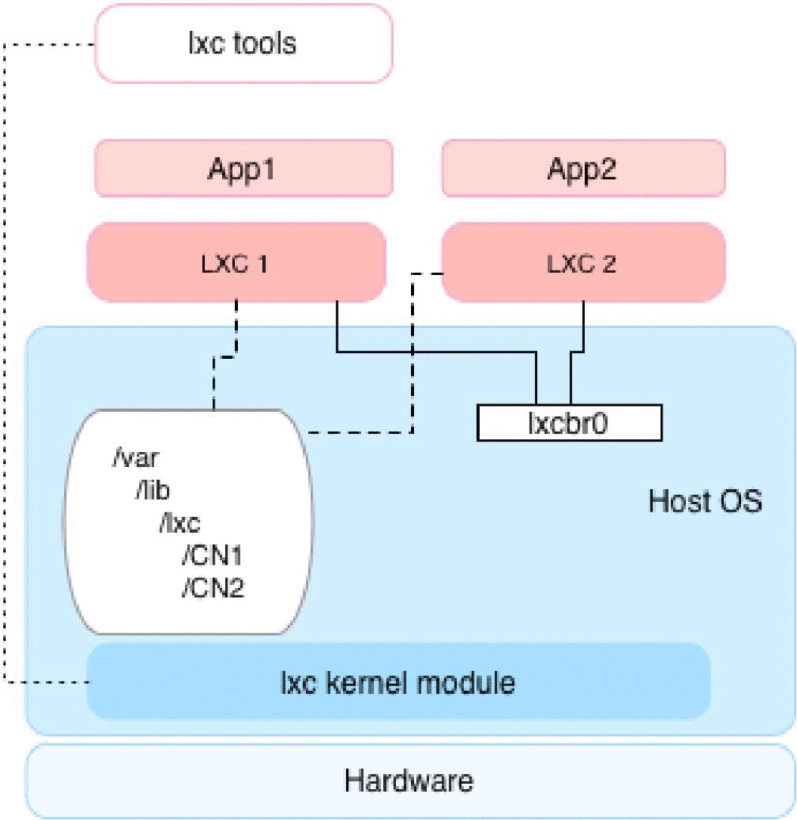
\includegraphics[width=0.5\textwidth]{images/3-containers.jpg}
  \caption{Zwei laufende LXC-Container in einer Linux Umgebung \cite{6903537}}
\end{figure}

\paragraph{}
\noindent Für andere Systeme bauen Container entsprechend auf anderen Features auf, das Prinzip lässt sich so aber auch auf andere Implementierungen übertragen

\paragraph{}
Es gibt verschiedene Ziele, die man mit einem Container erreichen will. Die zwei Hauptanwendungsfälle sind aber wohl OS-Container und Applikations-Container. Der Unterschied ist dabei aber kein technischer sondern mehr ein konzeptueller.\\
Ein OS-Container kann als virtuelle Maschine ohne Performance-Overhead betrachtet werden, die sich wie beschrieben den Kernel mit dem Host-System teilt. Die Container können, einmal gestartet, wie ein normales Betriebssystem bedient werden. Es können beliebig viele Container mit unterschiedlichsten Zielen auf einem System laufen. Zum Beispiel könnte man einen Container erstellen, auf dem man alle nötigen Services installiert, um eine Webanwendung laufen zu lassen. Lässt man den Container auf einem anderen Host-System laufen, sind wieder genau die gleichen Versionen der Programmiersprachen, wie zB. Ruby oder PHP, der genutzten Datenbank oder dem Webserver aber auch von wichtigen System-Libraries, installiert. Genauso vorstellbar sind aber auch spezialisierte Container für Webserver und Datenbank, die über die Linux Bridge miteinander kommunizieren \cite{ocvsac}. Die einzelnen Prozesse für die jeweiligen Services werden dabei in den jeweiligen Containern gestartet und nicht auf dem Host-System. So kann sichergestellt werden, dass man auf unterschiedlichen Host-Systemen die gleiche Webanwendung immer auf den gleichen Maschinen laufen lässt.

\begin{figure}[!ht]
  \centering
  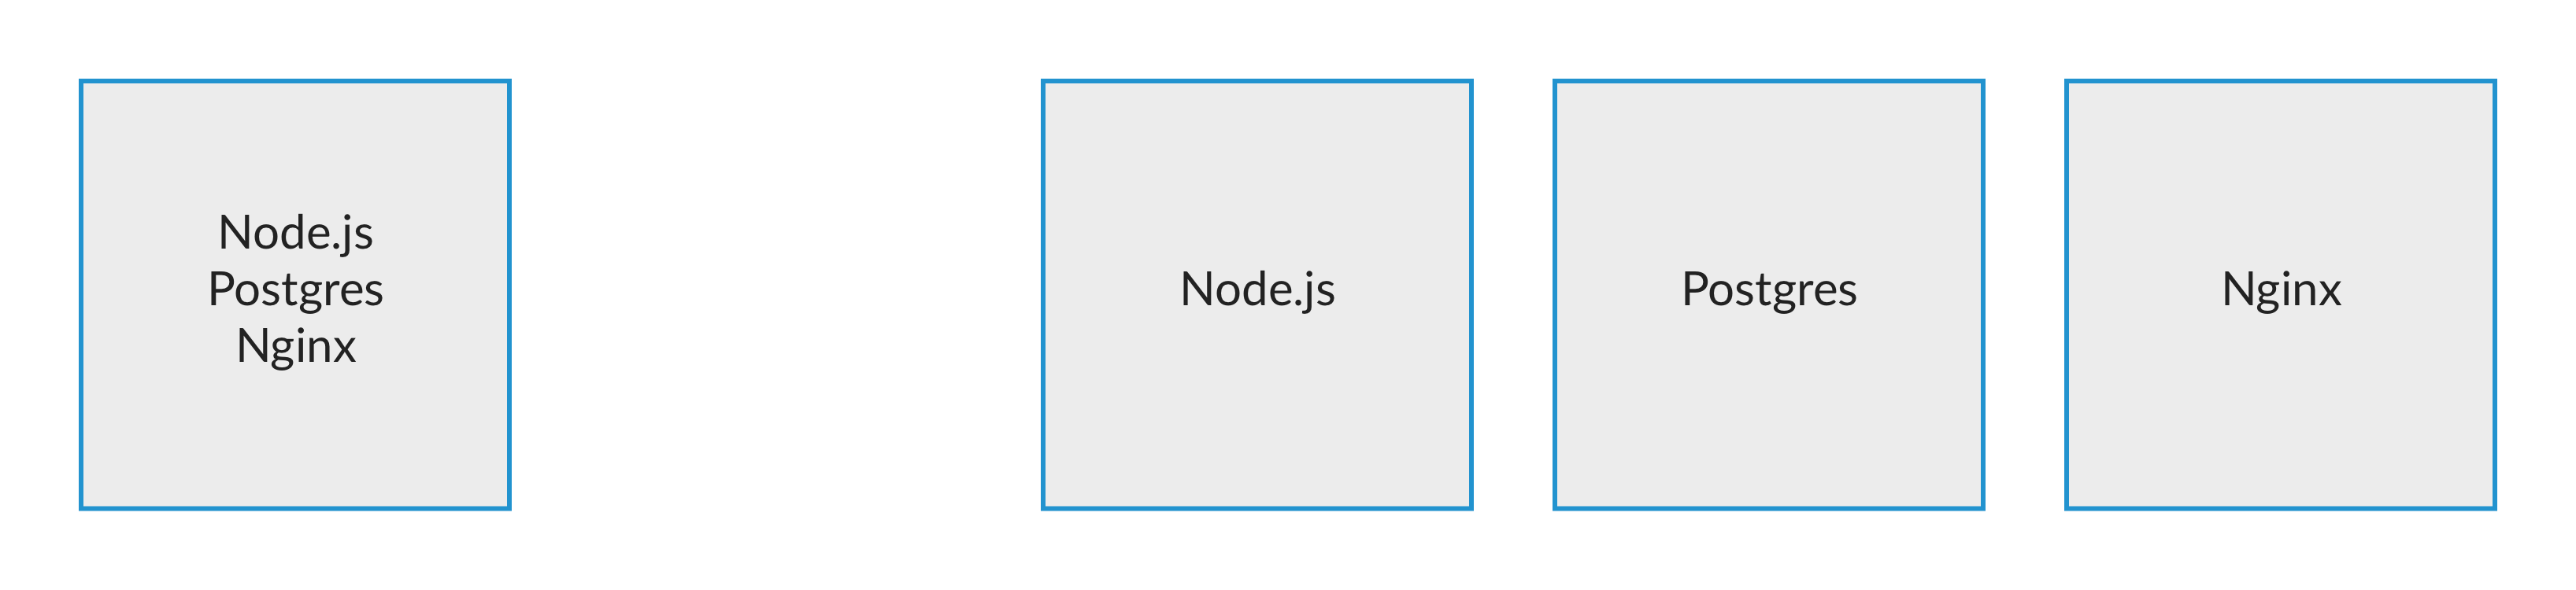
\includegraphics[width=1\textwidth]{images/4-os-specialized-containers.png}
  \caption{Ein OS-Container mit allen nötigen Services (links) und einzelne spezialisierte OS-Container (rechts)}
\end{figure}

Im Gegensatz zu OS-Containern wird mit einem Applikations-Container das Ziel verfolgt, ein Paket mit allen nötigen Abhängigkeiten zu erstellen, welches dann als einzelner Prozess auf einem beliebigen Host gestartet werden kann.
Applikations-Container bestehen oft aus sogenannten Layern, einzelnen Images die später beim Bauen des Images, welches zum Starten der Anwendung verwendet wird, zusammengefasst werden. Diese entsprechen den einzelnen spezialisierten Containern in dem oben genannten Beispiel. Der Vorteil ist, das die einzelnen Services in dem Fall im gleichen Namespace ausgeführt werden und dementsprechend aufeinander zugreifen können. Nutzt man Microservices als Architekturmuster ist es zum Beispiel sinnvoll, die einzelnen Services jeweils in Containern laufen zu lassen und die jeweiligen Layer in den verschiedenen Containern wiederzuverwenden.

\begin{figure}[!ht]
  \centering
  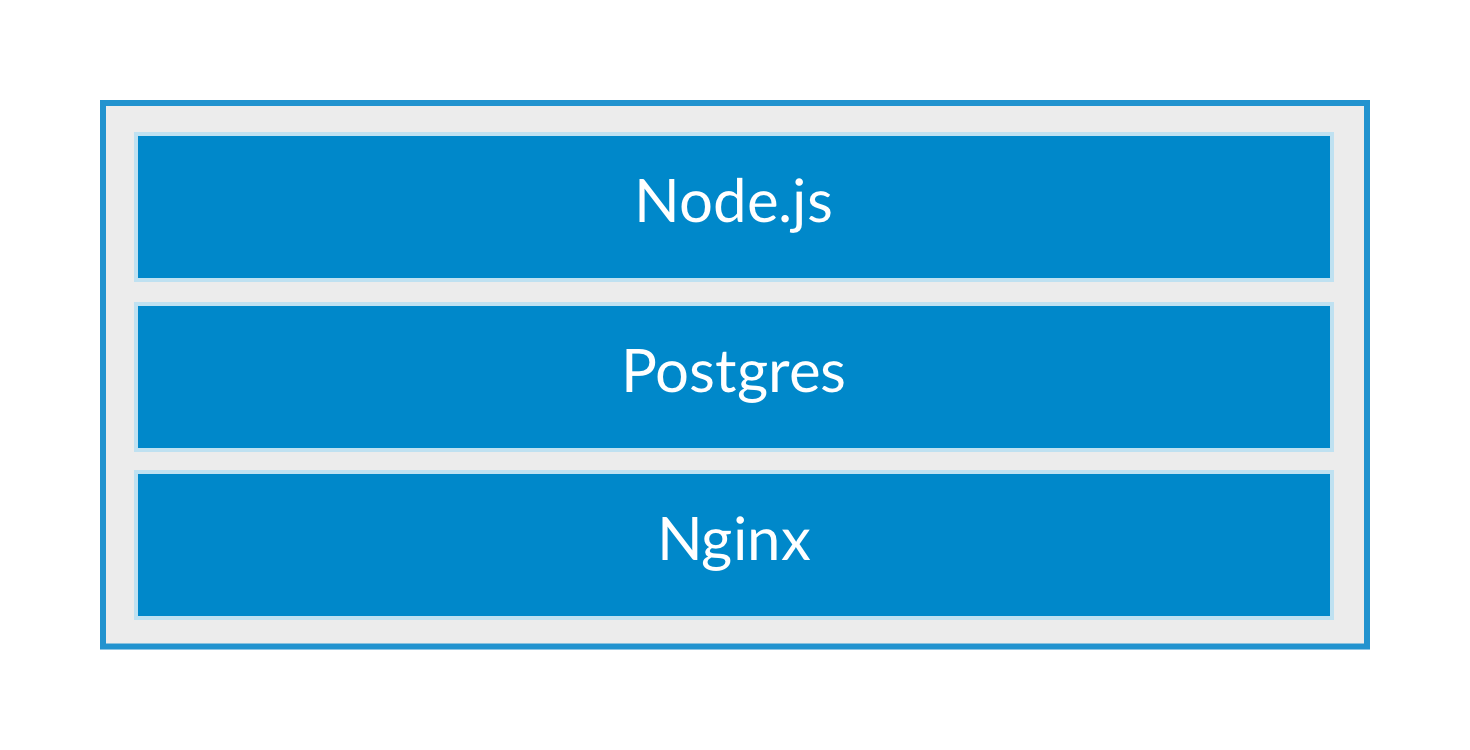
\includegraphics[width=0.6\textwidth]{images/5-application-container.png}
  \caption{Ein Applikations-Container mit mehreren Layern}
\end{figure}

% ---------
% Daemon
% ---------

\section{Daemon}
Als Daemon bezeichnet man unter Unix oder unixartigen Systemen ein Programm, das im Hintergrund abläuft und bestimmte Dienste zur Verfügung stellt. Der Benutzer interagiert dabei nicht direkt mit dem Programm, sondert indirekt über Ereignisse auf dem System. Das kann zum Beispiel eine Hardwareüberwachung sein, die überprüft ob ein Wechselmedium an das System angeschlossen wurden, aber auch ein Webserver, der auf Anfragen HTTP-Anfragen wartet \cite{wiki:daemon}.

\chapter{Container und VMs}

Container werden oft als “lightweight VMs” bezeichnet, was naheliegend ist, da beide Technologien darauf ausgelegt sind ein Betriebssystem zu simulieren, um eine Applikation in einer isolierten Umgebung laufen zu lassen, um die Applikationen portabel zu halten und Schäden am Host-System zu verhindern \cite{docker:cvsvm}.
Und doch haben beide Technologien wenig gemeinsam. Während im Falle der virtuellen Maschinen ein komplettes System mit Hardware, Betriebssystem und Applikation simuliert wird, reicht es für das Ausführen einer Applikation in einem Container Teile eines Betriebssystem zu simulieren.
Ein weiterer großer Unterschied ist, dass VMs einen Zustand haben. Sie repräsentiert ein komplettes System mit Prozessen und Daten, das woanders wieder in genau diesem Zustand weiterlaufen kann. Erzeugt man eine weitere Instanz dieser Maschine ist es einfach nur eine genaue Kopie derselben Maschine. Container hingegen sind meist zustandslos.\\

\begin{figure}[!ht]
  \centering
  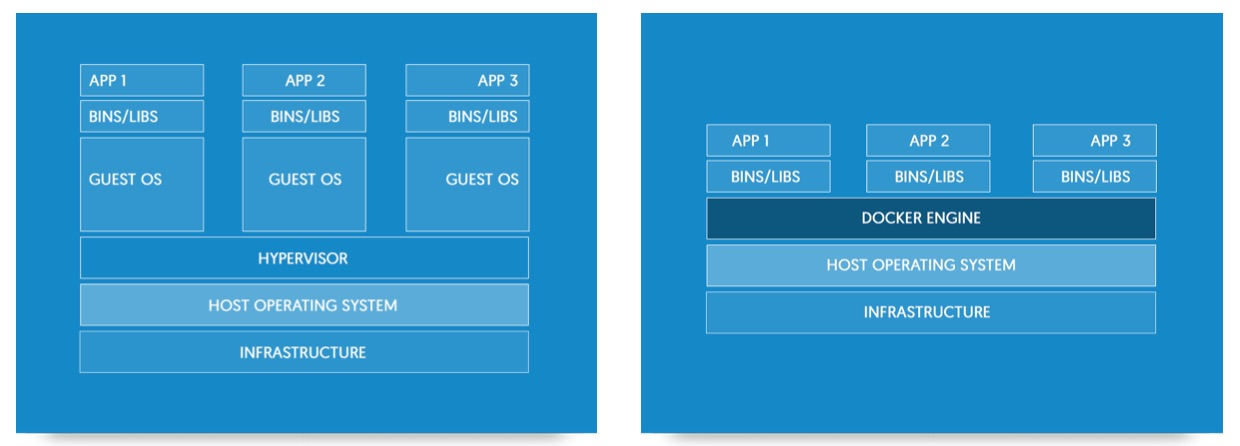
\includegraphics[width=0.8\textwidth]{images/container-vm.jpg}
  \caption{Verschiedene VMs und Container auf einem Host-System im Vergleich \cite{docker}}
\end{figure}

% Eventuell Performance (http://ieeexplore.ieee.org.ieeexplore.emedien3.sub.uni-hamburg.de/xpls/icp.jsp?arnumber=7092949) und Sicherheit (http://ieeexplore.ieee.org.ieeexplore.emedien3.sub.uni-hamburg.de/xpls/icp.jsp?arnumber=7432984)

\noindent Es gibt keine Regeln dafür, wann eine Applikation innerhalb eines Containers und wann sie innerhalb einer VM laufen sollte. Das kommt auf die Applikation an und muss von Fall zu Fall betrachtet werden. Bei einer monolithischen Webanwendung, also einer, die alle nötigen Services und Komponenten, wie Frontend, Backend und die Datenbanken, beinhaltet, macht es Sinn diese in einer virtuellen Maschine zu starten. Besteht die Anwendung aus vielen kleinen spezialisierten Microservices, macht es Sinn diese in einzelnen Containern zu starten. Grundsätzlich schließen sich beide Technologien aber auch nicht aus, da Container auf allen Host-Systemen gestartet werden können, die auf dem gleichen Kernel aufbauen - also auch virtuellen Maschinen. Sollen Anwendungen die in Containern laufen beispielsweise mit älteren, in VMs laufenden Anwendungen zusammenarbeiten, bei denen klar ist, dass diese nicht noch einmal überarbeitet werden sollen , können diese einfach mit auf der VM gestartet werden. So können die Vorteile beider Technologien miteinander kombiniert werden \cite{docker:cavm}.\\

\begin{figure}[!ht]
  \centering
  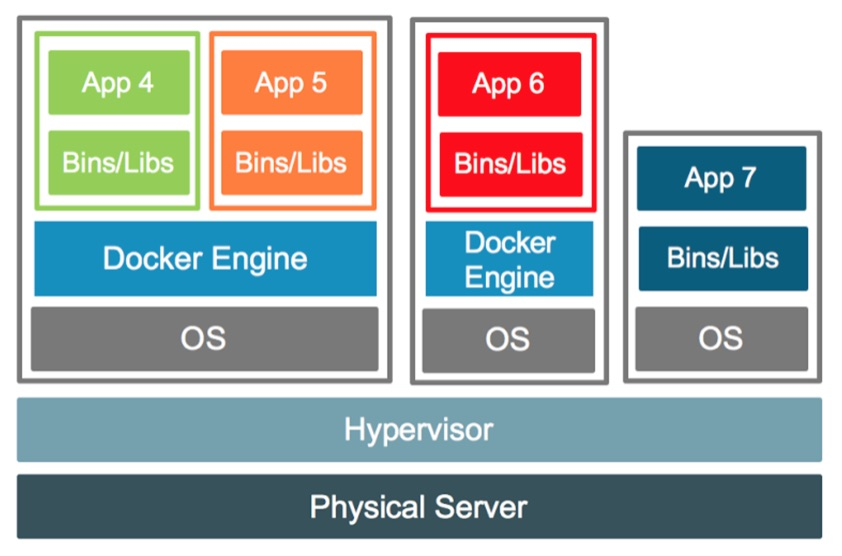
\includegraphics[width=0.6\textwidth]{images/container-vm-combined.jpg}
  \caption{VMs und Docker Container kombinier \cite{docker:cavm}}
\end{figure}

\chapter{Docker}

Docker soll es Entwicklern vereinfachen, Container für Applikationen zu erstellen, zu verteilen und sie auf verschiedensten Systemen auszuführen. Es hilft dabei Applikations-Container zu erstellen \cite{docker}, die später in einem einzelnen Prozess auf verschiedenen Systemen ausgeführt werden können. Die erste Version wurde im März 2013 von dotCloud veröffentlicht (jetzt Docker, Inc.) \cite{docker:rel}.
Docker basierte bis zu Version 0.9 \cite{docker:cl} auf dem Container-Standard LXC und erweiterte diese vor allem durch eine einfachere Handhabung. So können Images durch einfache Konfigurationsdateien definiert werden und über die Docker API erstellt und verwaltet werden. Beim Starten eines Containers können diese mit anderen verbunden werden, um so die Kommunikation der eigentlich voneinander isolierten Container zu vereinfachen und über andere Tools können ganze Cluster von Docker-Containern verwaltet werden.

\paragraph{}
Über eine Docker-Registry ist es möglich Container Images zu versionieren und zu teilen. Die Docker-Registry kann wie Git für Container gesehen werden.  Bei dem Bau neuer Container Images kann man so immer wieder auf sogenannte Base-Images zurückgreifen, die man in einer Docker-Registry findet und auf denen man seine eigenen Images aufbauen kann.

\paragraph{}
LXC ist dabei nur ein Tool um Container zu erstellen und zu starten und Docker vereinfacht die Verwaltung dieser Container. Mit “libcontainer” implementierte Docker Inc. eine eigenen Container-Standard, um die starken Abhängigkeiten von LXC aufzulösen. Daraus ging die “Open Container Initiative”, die OCI (https://www.opencontainers.org/) und “runC” (http://runc.io/) hervor. Die OCI ist ein Zusammenschluss mehrerer großer Firmen, angeführt von Docker, mit dem Ziel, einen einheitlichen offenen Container Standard zu definieren. Anhand dieser Spezifikation können Container dann auf verschiedenen Systemen implementiert werden und von Systemen wie Docker einheitlich verwaltet werden. runC ist dabei die Implementation der Spezifikationen der OCI und ersetzt LXC.

% ------------
% -- Engine --
% ------------

\section{Docker Engine}

Die Docker Engine ist eine Client-Server Anwendung, die auf dem Host-System installiert wird und besteht aus drei Hauptbestandteilen:\\

\begin{itemize}
  \item dem Docker Daemon (der Server), der für das Erstellen und Ausführen der Container zuständig ist
  \item der Docker Remote Api für die Kommunikation zwischen Client und Docker Daemon
  \item der CLI (Command Line Interface)
\end{itemize}

\begin{figure}[!ht]
  \centering
  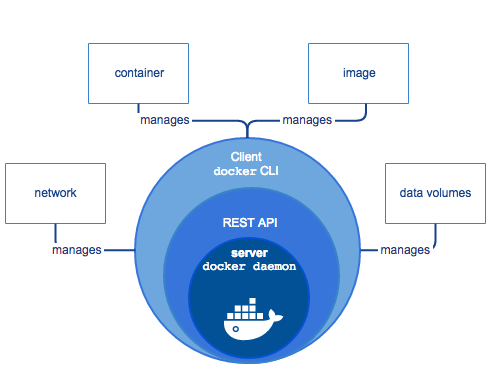
\includegraphics[width=0.5\textwidth]{images/docker-engine.png}
  \caption{Die drei Hauptbestandteile der Docker-Engine \cite{docker:ud}}
\end{figure}

Die Client-Server Architektur ermöglicht es einerseits Client und Daemon auf verschiedenen Hosts laufen zu lassen und so auch Container auf anderen Servern zu verwalten, andererseits kann der Daemon durch die API über einen beliebigen Client gesteuert werden. Das können andere Sprachen wie beispielsweise Python sein, für die eine vollständige Docker-Api-Implementation vorliegt oder auch grafische Benutzeroberflächen.

% --------------------------
% -- Images and Container --
% --------------------------

\section{Images und Container}

Ein Docker Container wird auf Basis eines Docker Images gebaut. Jedes Docker Image besteht aus mehreren Layern, einem Base Image und welchen, die das Image jeweils um Funktionen erweitern, die für das Ausführen einer Applikation wichtig sind. Die Layer liegen dabei in jeweils eigenen Verzeichnissen und werden über ein “unified view” zu einem einzelnen Image zusammengefasst. Ein “unified view” kann als virtuelles Verzeichnis gesehen werden, in dem die einzelnen Layer so übereinandergelegt werden, dass die verschiedenen Layer von oben als einzelnes Image gelesen werden können. Existiert in einem Layer die gleiche Datei wie in dem Base Image mit einer anderen Konfiguration, so verdeckt diese die Datei aus dem Base Image.\\

\begin{figure}[!ht]
  \centering
  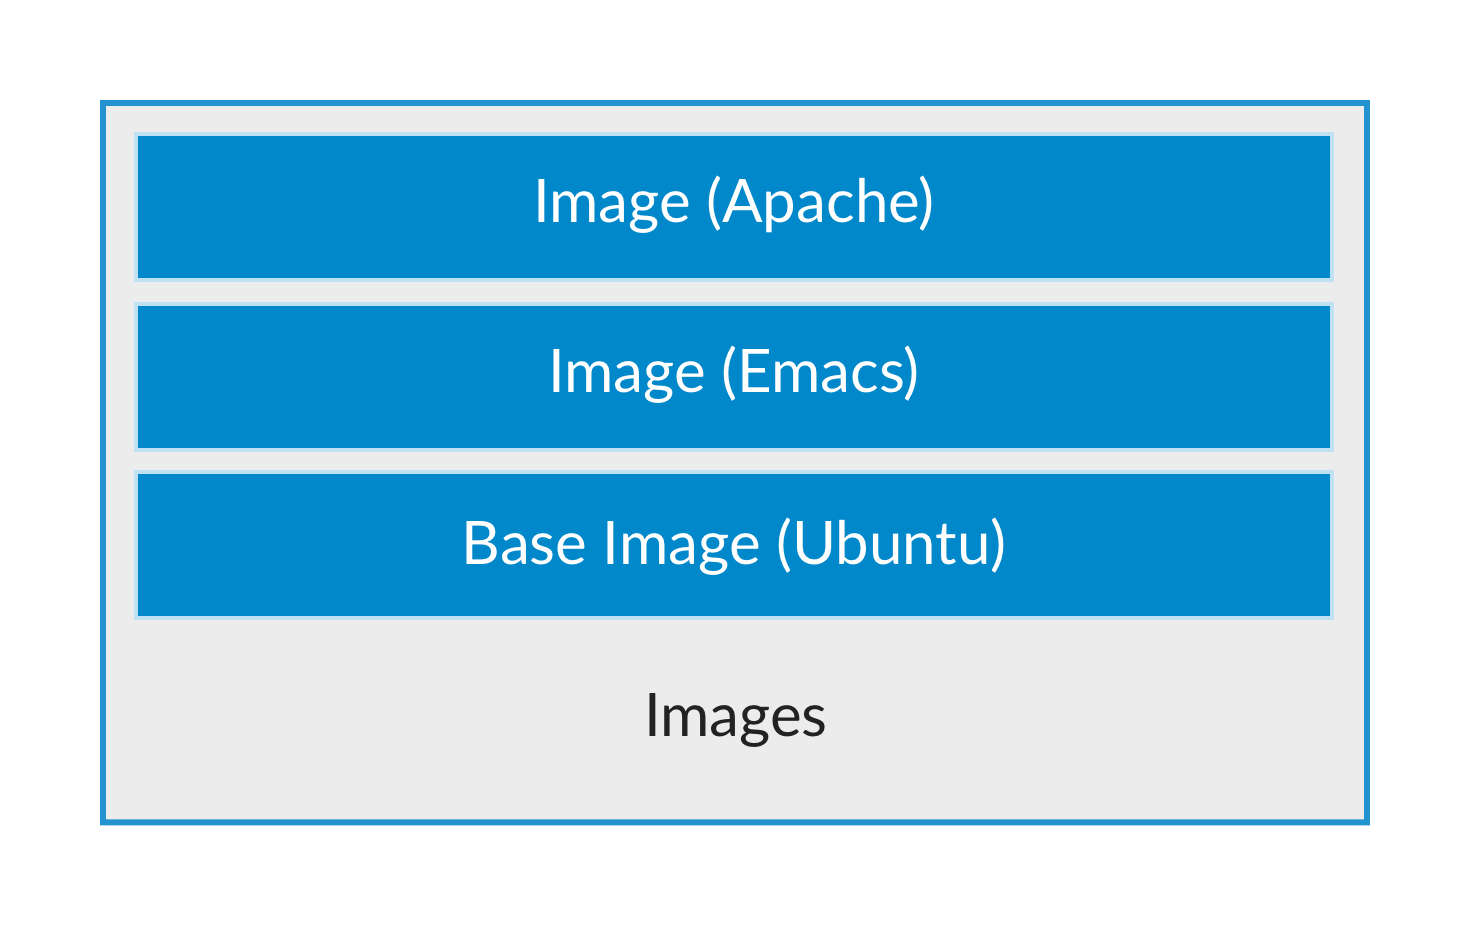
\includegraphics[width=0.6\textwidth]{images/docker-image.png}
  \caption{Ein Image bestehend aus mehreren übereinandergestapelten Layern \cite{7158965}}
\end{figure}

Die einzelnen Layer in einem Image sind nur lesbar, können also nicht mehr verändert werden. So können die Layer von beliebig vielen Images verwendet werden. Jeder Layer hat einen eindeutigen Hash und kann gezielt von verschiedenen Images verwendet werden und es kann sichergestellt werden, dass der Layer immer genau gleich ist. Das bedeutet, dass der Layer nur ein einziges Mal im Dateisystem gespeichert werden muss. Über die “unified view” werden die Layer anschließend in den Images verwendet. So können die Layer von beliebig vielen Images verwendet werden bei konstantem Platzverbrauch. Jede Änderung an einem Image fügt dem Image einen Layer hinzu. Jeder Layer steht dabei für Unterschiede im Dateisystem im Bezug auf die übrigen Layer. Das können nur einzelne Konfigurationsdateien sein, sodass die Größe des Layers nur wenige Bytes beträgt, aber auch ganze Programmpakete, die deutlich mehr Platz benötigen.\\

\begin{figure}[!ht]
  \centering
  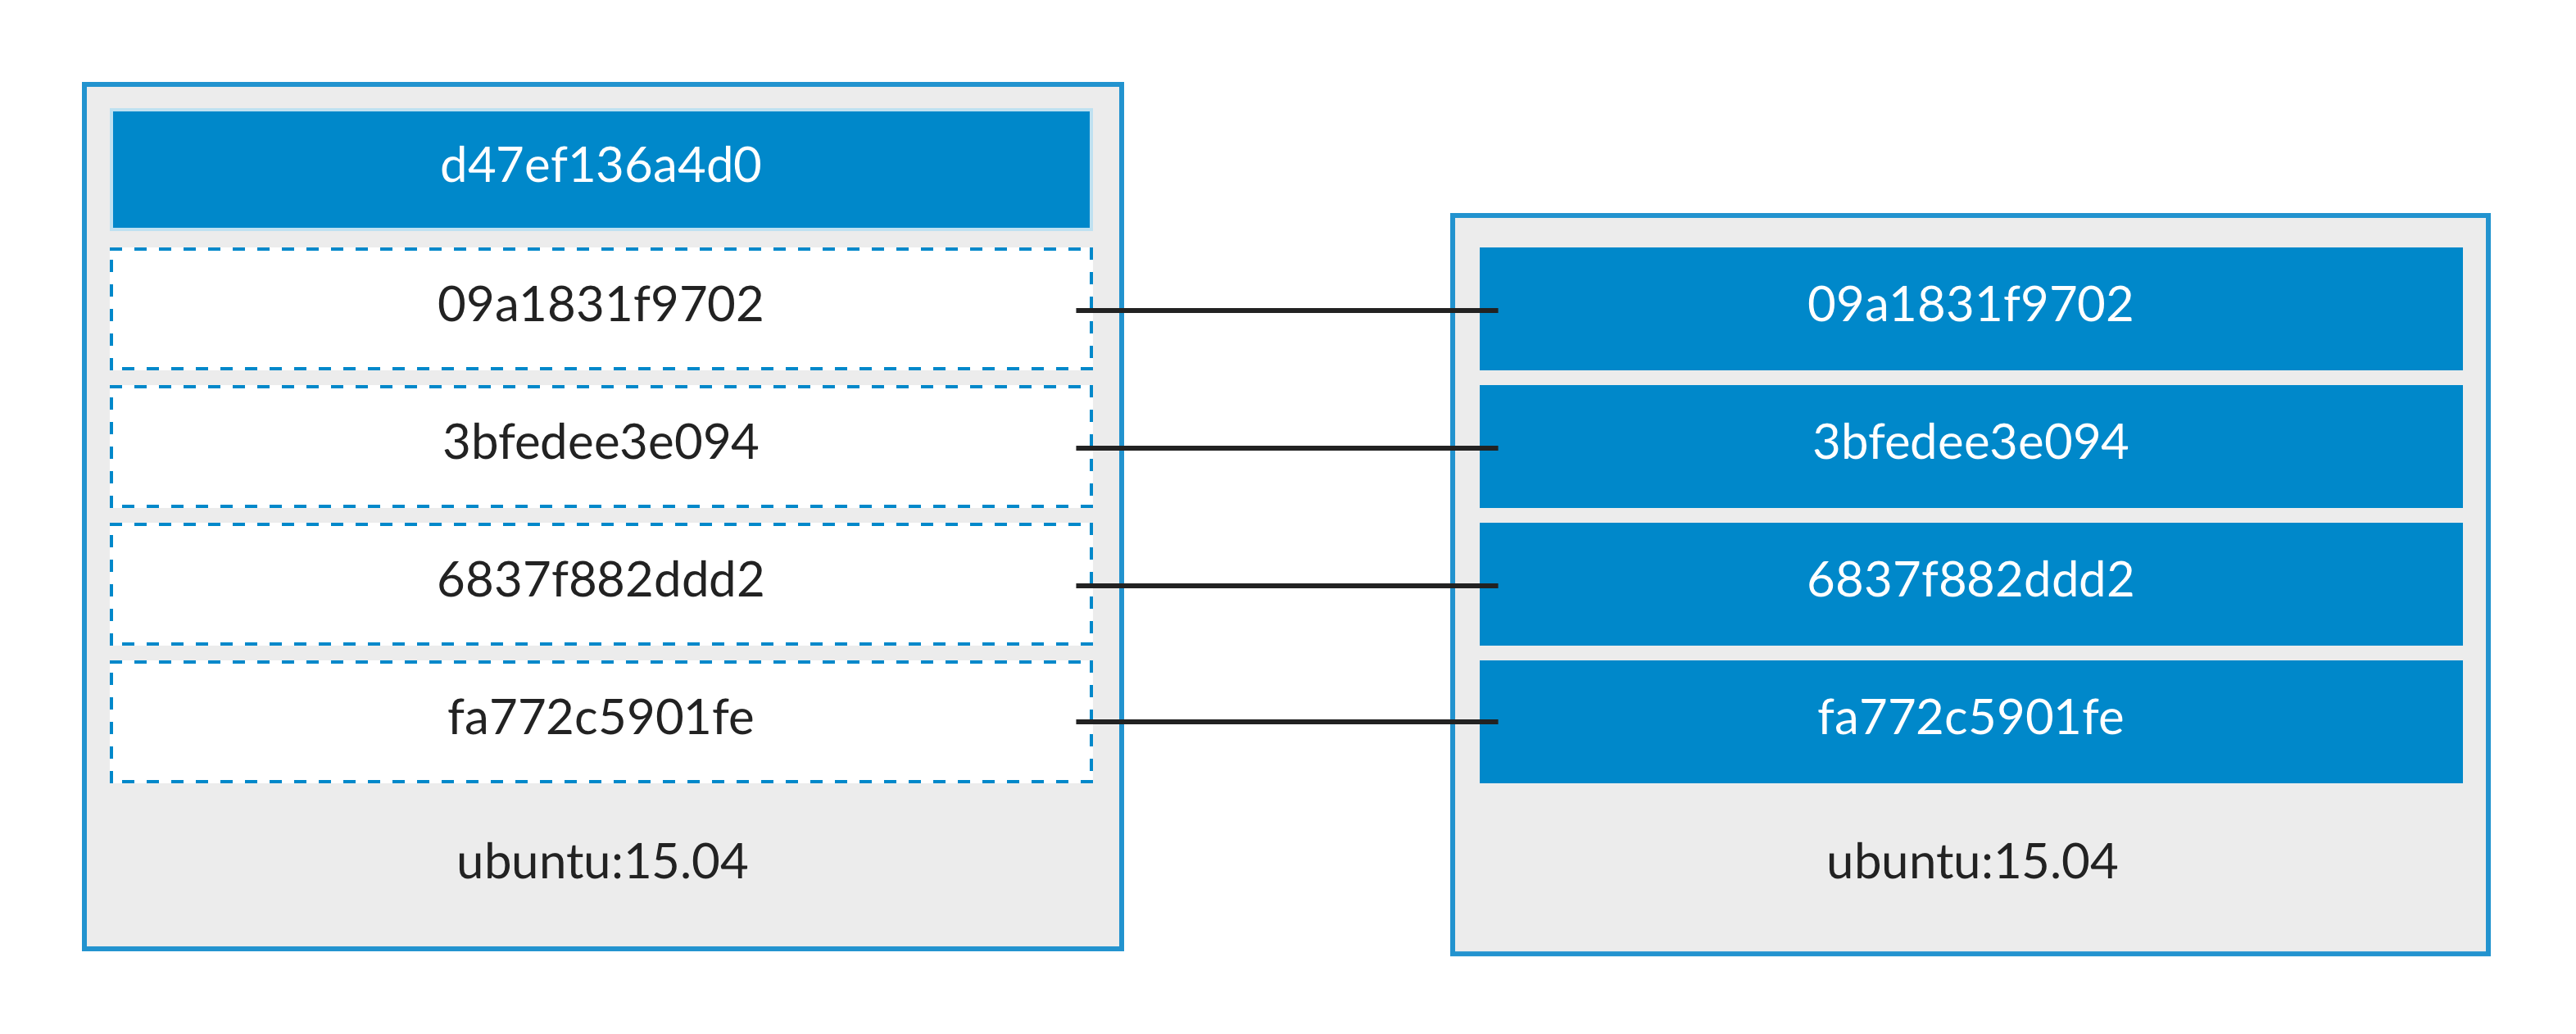
\includegraphics[width=1\textwidth]{images/docker-image-layer-sharing.png}
  \caption{Ein Image mit neuem Layer, dass die ursprünglichen Layer mit verwendet \cite{docker:images}}
\end{figure}

Bei der Erstellung eines Containers aus einem Image wird nach dem gleichen Prinzip dem ursprünglichen Image nun ein “Container-Layer” hinzugefügt, der im Gegensatz zu den übrigen beschreibbar ist. Ist der Container gestartet, werden alle Dateiänderungen in den diesen Layer geschrieben. Dafür ist neben dem “Unified View” ist noch ein weiteres Verfahren, das “copy-on-write” Verfahren wichtig. Während die Container laufen, arbeiten beliebig viele Container mit den gleichen Original-Dateien aus dem jeweiligen Layern. Da diese nur gelesen werden können, können diese entsprechend nicht von den jeweiligen Containern modifiziert werden. Deshalb werden diese Dateien, sobald sie verändert werden sollen aus dem jeweiligen Read-Only Layer in den Container-Layer kopiert, wo sie entsprechend bearbeitet werden können.
Der Container, der die Datei bearbeitet hat arbeitet danach mit seiner Kopie im Container-Layer, während die übrigen Container weiter mit dem Original arbeiten. Dadurch können beliebig viele Container platzsparend zur gleichen Zeit laufen \cite{docker:images}.\\

\begin{figure}[!ht]
  \centering
  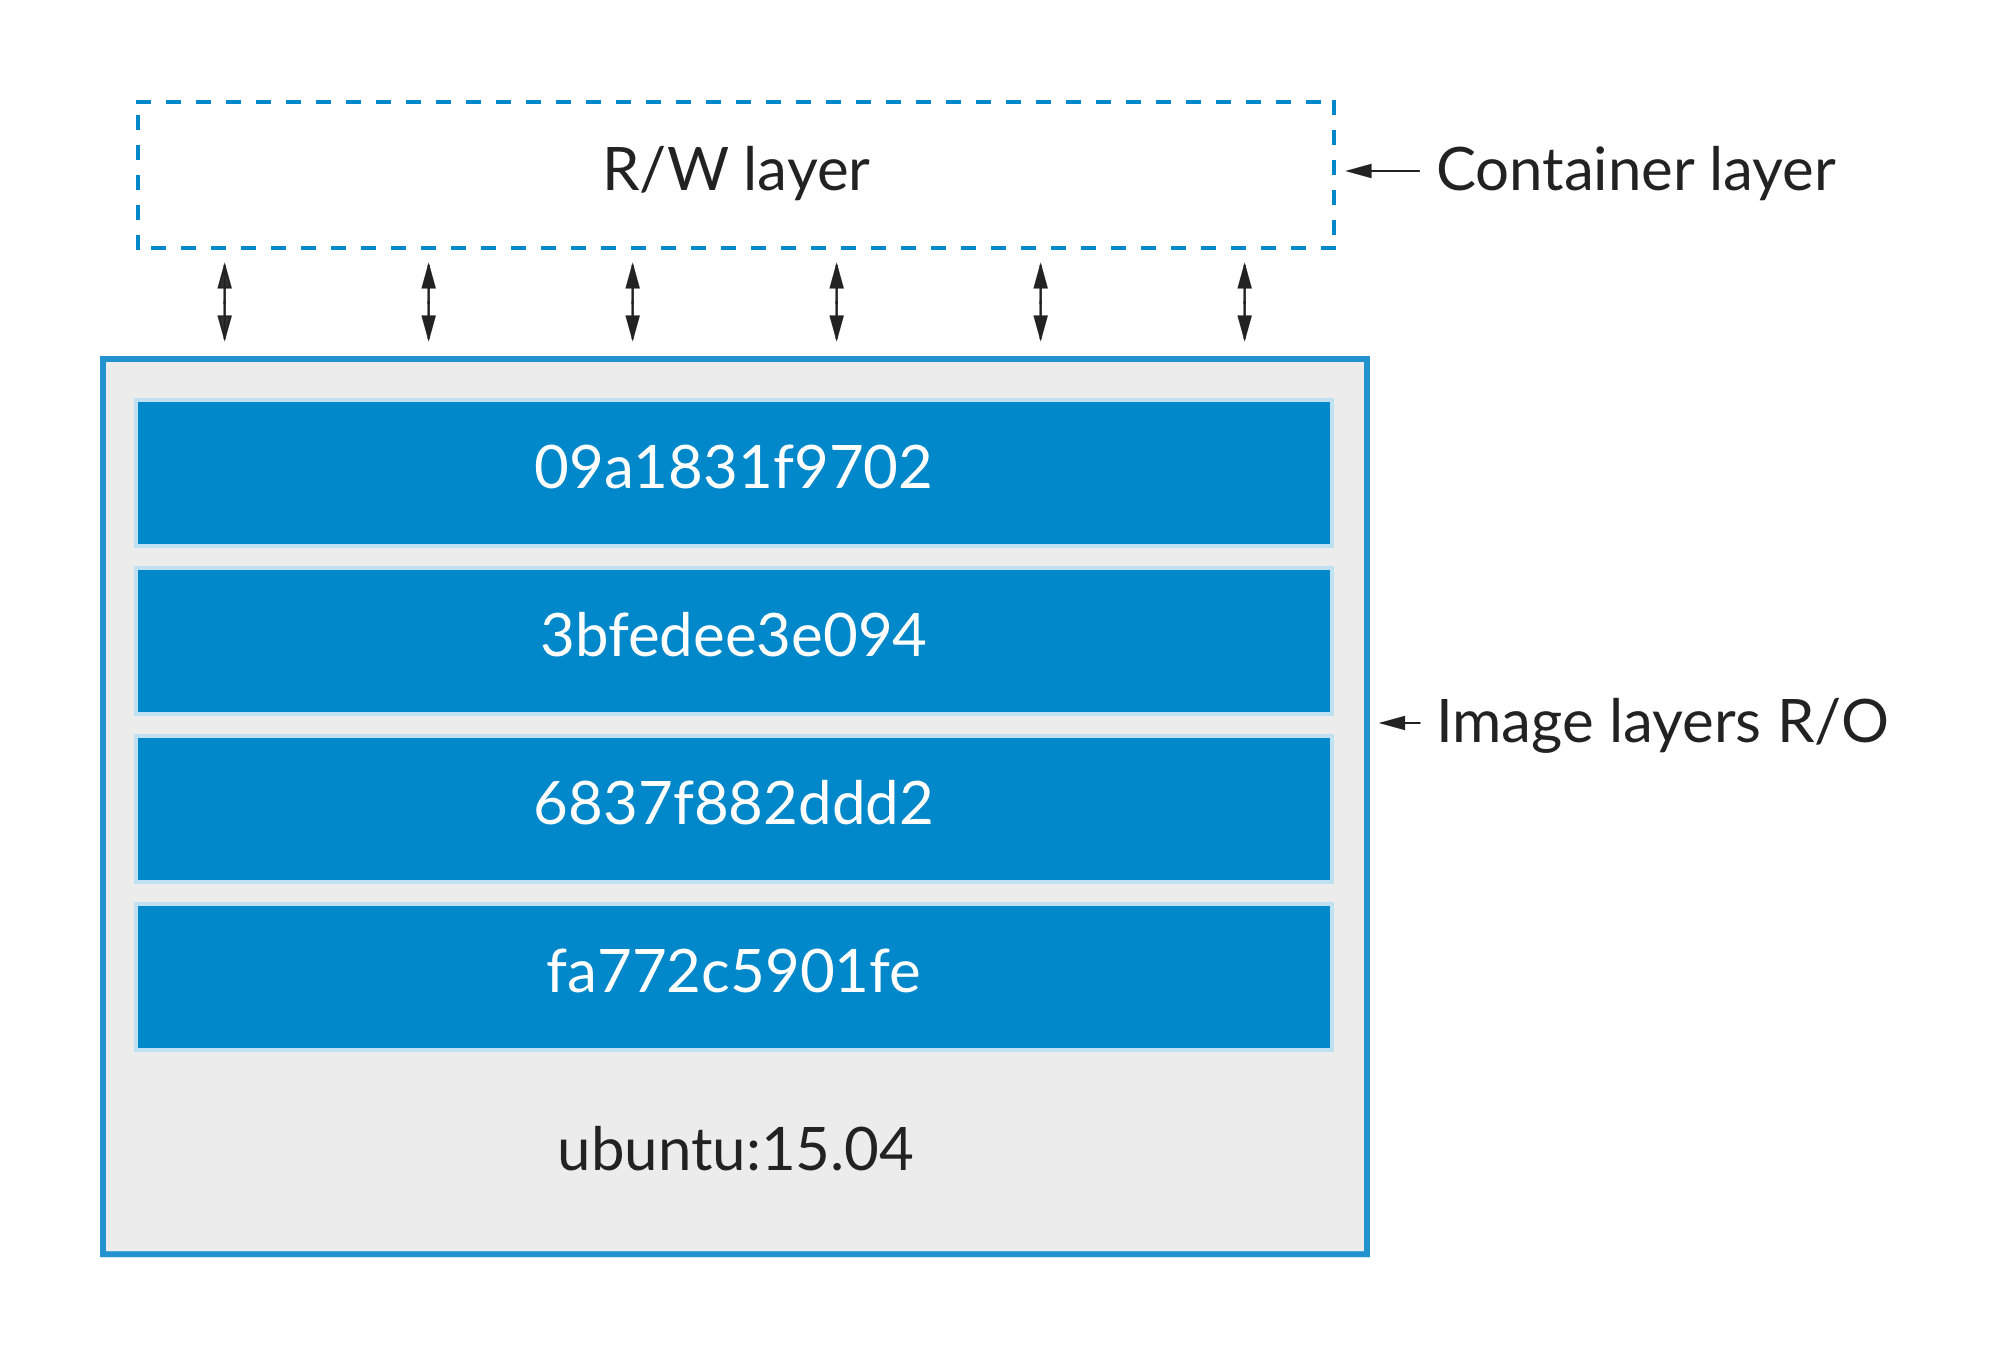
\includegraphics[width=0.8\textwidth]{images/docker-container.png}
  \caption{Ein Container, bestehend aus R/O Image Layern und R/W Container Layer \cite{docker:images}}
\end{figure}

Gesteuert werden sowohl der “Unified View” als auch “Copy-on-Write” von verschiedenen “Storage-Drivern”, die zwar unterschiedlich implementiert sind, aber auf dem gleichen Prinzip beruhen. Bei der Konfiguration von Docker, kann man zwischen verschieden Implementierungen wählen. Die bekanntesten sind wohl “auFS” und “overlayFS”.

\paragraph{}
Beim Löschen  eines Containers werden auch alle Dateien, die beim Ausführen der Applikation erstellt wurden, gelöscht. Für das Persistieren von Daten gibt es die Möglichkeit, die Container mit sogenannten Data-Volumes zu verbinden.

\paragraph{}
Definiert werden die Images über Dockerfiles. Vereinfacht fügt jeder Befehl in der Datei dem Image ein neuen Layer hinzu. Über "docker build" wird das Image entsprechend des Dockerfiles gebaut. Jedes Image kann auf bereits vorhandenen Images aufbauen. Images können in einer Docker-Registry gespeichert werden und werden bei Bedarf bei der Erstellung des Images heruntergeladen. Dabei werden bereits vorhandene Layer im Dateisystem nicht erneut heruntergeladen. Das Beispiel baut ein Image basierend auf Ubuntu, das beim Starten des Containers “Hello world” ausgibt und in eine Datei schreibt.\\

\begin{figure}[!ht]
  \centering
  \sourcecode{src/Dockerfile1}
  \caption{Ein Dockerfile}\label{figure:Dockerfile}
\end{figure}

% --------------------------
% ----- Docker Daemon ------
% --------------------------

\section{Docker Daemon}

Der Docker Daemon (dockerd\footnote{https://docs.docker.com/engine/reference/commandline/dockerd/}) ist der zentrale Bestandteil von Docker. Er ist die Schnittstelle zwischen der einfachen Handhabung von Docker und den Vorteilen Applikations-Container gegenüber normalen VMs bieten. Er setzt auf containerd\footnote{https://containerd.io/} auf, einer Ausführungsumgebung(runtime) für Container, um runC Container nach dem OCI-Standard auszuführen und zu verwalten. containerd basiert auf Dockers altem Daemon. Er setzt auf einem niedrigeren Level an und wird von dem Docker Daemon erweitert. Wird der Docker Daemon über seine API angesprochen gibt dieser die vereinfachten Befehle übersetzt an containerd weiter \cite{docker:daemon}.\\

% https://blog.docker.com/2016/04/docker-engine-1-11-runc/, https://docs.docker.com/engine/understanding-docker/
\begin{figure}[!ht]
  \centering
  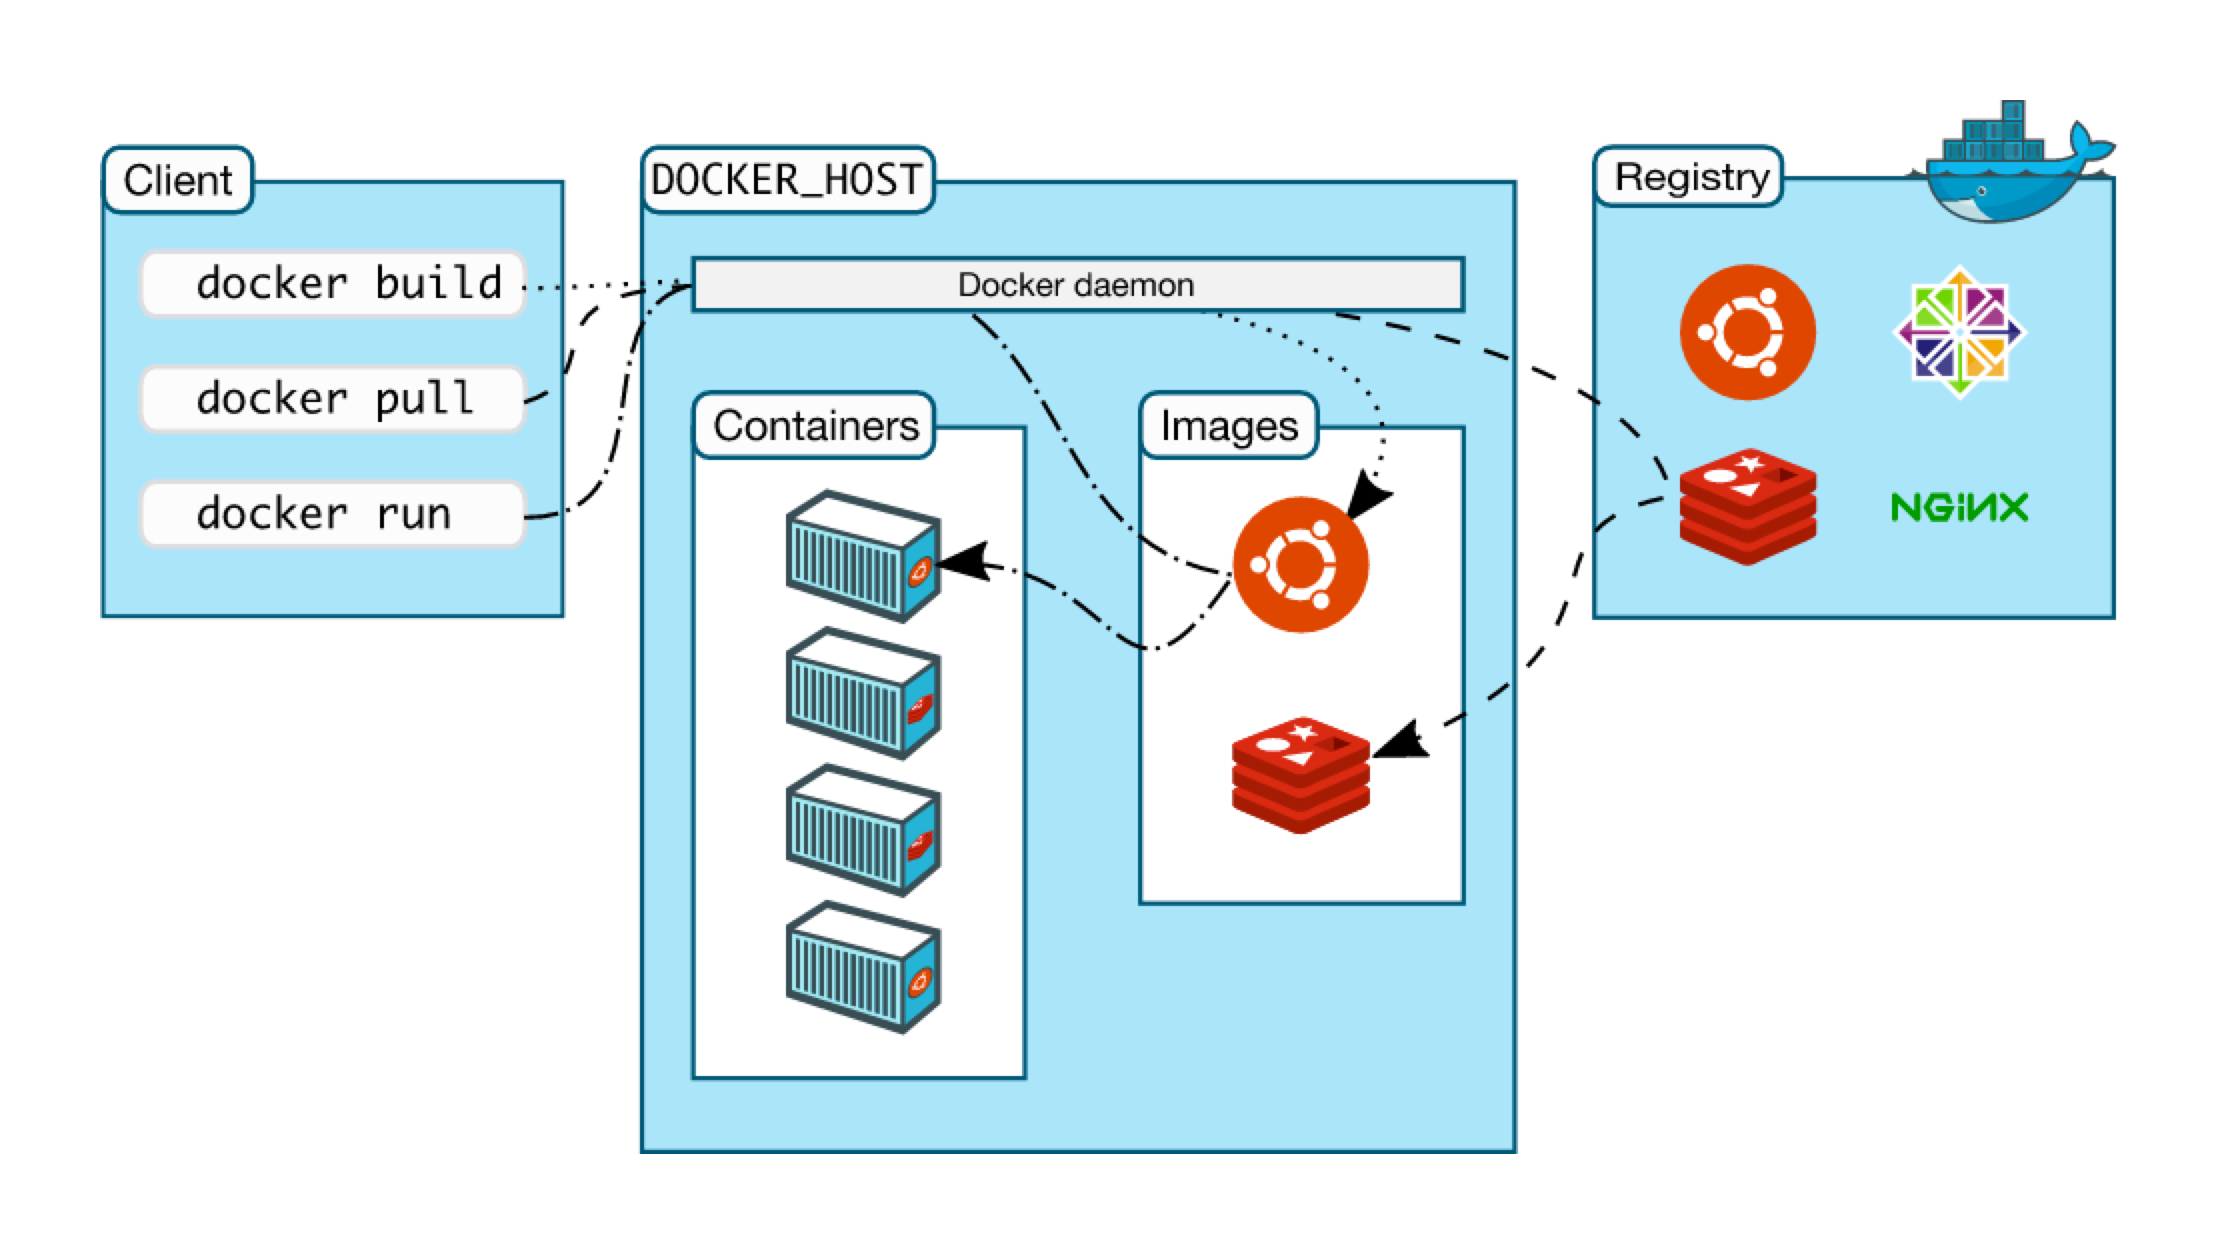
\includegraphics[width=0.8\textwidth]{images/docker-daemon.png}
  \caption{Docker Daemon\cite{docker:ud}}
\end{figure}

\noindent Wird zum Beispiel das Kommando \code{docker run -i -t ubuntu} ausgeführt, checkt die Docker Engine, ob das Ubuntu Image sich bereits auf dem System befindet. Ist das nicht der Fall wird das Image aus der Docker Registry gepullt und auf die Festplatte geladen. Daraus wird der Container erstellt, indem dem Image ein R/W Layer hinzugefügt wird. Danach wird das Netzwerk entsprechend konfiguriert, damit der Docker Container mit dem Host-System kommunizieren kann und dem Container wird eine IP-Adresse zugewiesen, über die der Container erreichbar ist. Zum Schluss werden die definierten Kommandos aus dem Dockerfile ausgeführt und man kann (durch das \code{-i} Flag) über das Terminal mit dem Container interagieren.

% -------------------------
% ------ Docker API -------
% -------------------------

\section{Docker API}
Über die Docker Remote API kann ein Client mit dem Docker Daemon ansprechen. Client und Daemon können sowohl auf dem gleichen Host als auch über verschiedene Hosts über die Http-Schnittstelle miteinander kommunizieren. Der Client muss dabei kein Benutzer sein, sondern können zum Beispiel Überwachungsprogramme sein. Unter anderem bietet die Docker API zum Beispiel einen Event-Stream, bei dem sich diese Programme registrieren und dementsprechend auf Zustandsänderungen reagieren können. Fällt zum Beispiel ein Container aus, können so automatisch neue Container erstellt und ausgeführt werden \cite{docker:api}.\\

\begin{figure}[!ht]
  \centering
  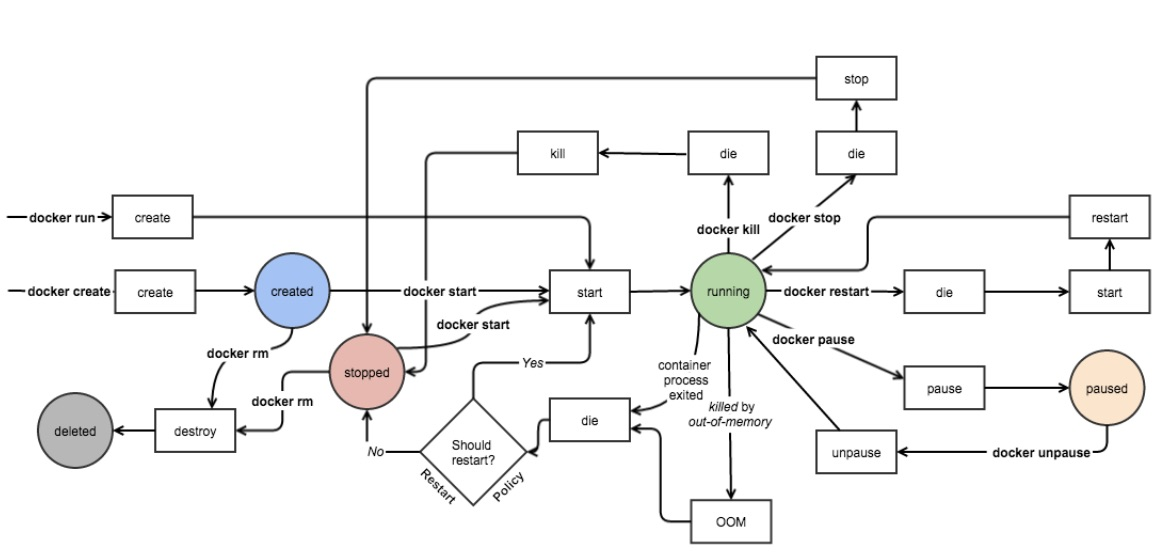
\includegraphics[width=0.8\textwidth]{images/docker-api.jpg}
  \caption{Die Zustände die ein Docker-Container besitzen kann und die dafür verantwortlichen Events \cite{docker:api}}
\end{figure}

% -------------------------
% ------ Docker CLI -------
% -------------------------

% \section{Docker CLI}
%
% Über die Docker CLI kann man den Docker Daemon über die Docker Remote API ansprechen. Hier einige wichtige Befehle:\\
%
% \begin{itemize}
%   \item \code{docker build}
%   \item docker run
%   \item docker build
%   \item docker start
%   \item docker push
%   % \item docker rm CONTAINER_ID
%   % \item docker rmi IMAGE_ID
%   % \item docker images
%   \item docker ps -a
%   \item ...
% \end{itemize}

\chapter{Fallbeispiel}

\begin{figure}[!ht]
  \centering
  \sourcecode{src/Dockerfile2}
  \caption{Ein Dockerfile}\label{figure:Dockerfile}
\end{figure}

Workdir wird mit in container geladen und kann ausgeführt werden, lokal volume sodass man app entwickeln kann

\begin{figure}[!ht]
  \centering
  \sourcecode{src/docker-compose.dev.yml}
  \caption{Docker-Compose Development}\label{figure:docker-compose development}
\end{figure}

Baut images db und web, db aus iamge, web nach Anleitung aus Dockerfile.
docker-compose up baut images und spawnt container

docker-compose build, docker push kddc/dbaas_web, docker push kddc/dbaas_db
pusht neuste container in docker registry.

\begin{figure}[!ht]
  \centering
  \sourcecode{src/docker-compose.prod.yml}
  \caption{Docker-Compose Production}\label{figure:docker-compose production}
\end{figure}

Auf Server anderes docker-compose script, zieht sich images startet container port 80

\chapter{Fazit}

Die Einsatzmöglichkeiten von Containern sind vielfältig. Sie erleichtern die Portierbarkeit von Anwendungen, sparen Platz und schonen die Ressourcen. Sie können Entwicklern dabei helfen, Fehlverhalten in ihrer Anwendung aufgrund unterschiedlicher Softwareversionen zu verhindern oder aber bei Bedarf in sehr kurzer Zeit beliebig viele Container zu einem Cluster von bestimmten Anwendungen oder Services zuzuschalten, um das System zu entlasten. Der einfachste Fall ist wohl eine einfache monolithische Webanwendung, die leicht transportiert und auf nahezu jedem System einfach ausgeführt werden kann. Jedoch laden Container dazu ein, eine Software in Microservices aufzuteilen, damit die jeweiligen Services möglichst isoliert von anderen Bestandteilen der Software arbeiten können und sich nicht etwa durch die Abhängigkeiten von den gleichen Bibliotheken in verschiedenen Versionen ausbremsen. Diese Kleinteiligkeit stellt Entwickler aber auch wieder vor neue Herausforderungen. Zwar sind die Container im einzelnen leicht portierbar und werden stabil in ihrer isolierten Umgebung laufen, aber sie müssen auch mit den anderen Services einer Anwendung verknüpft werden oder im entsprechenden Cluster einsortiert werden, um das volle Potential auszuschöpfen.\\

\noindent Docker-Swarm\footnote{https://www.docker.com/products/docker-swarm} ist ein internes Tool in der Docker-Engine das bei der Orchestrierung der Container hilft, also unter welchen Voraussetzungen welche Cluster hochskaliert werden, wann Container abgeschaltet werden oder dem Austausch von defekten Containern.
Aber auch für diesen Zweck gibt es bereits Cloud Computing Services, über die das Verwalten von Containern bzw. Container-Clustern vereinfacht wird. Was Infrastructure as a Service (IaaS) für virtuelle Server und Platform as a Service (PaaS) für fertige Laufzeitumgebungen ist, ist Container as a Service (CaaS) für Container. CaaS ist irgendwo zwischen IaaS und PaaS anzusiedeln, ähnelt aber vor allem IaaS, mit dem Unterschied, dass Container und nicht virtuelle Maschinen die vermieteten Ressourcen sind. Die CaaS Plattformen helfen dabei vor allem bei der Orchestrierung der Container. Bekannte Anbieter sind vor allem Amazon EC2 Container Service\footnote{https://aws.amazon.com/de/ecs/} und Google Kubernetes\footnote{https://kubernetes.io/}.\\

\newpage

\noindent Zusammenfassend lässt sich sagen, dass das Prinzip von Containern zwar schon länger bekannt ist, aber erst seit einigen Jahren erfährt die Technologie vermehrt Beachtung, da durch Unternehmen wie Docker endlich eine vereinfachte Schnittstelle für Entwickler geschaffen wurde, um mit Containern zu arbeiten. Es gibt zwar noch einige kritische Stimmen, die vor allem Bedenken wegen der Sicherheit von Containern äußern, dennoch bergen sie vor allem viele Möglichkeiten für Entwickler ihre Anwendungen stabiler und flexibler zu gestalten.\\
%
% \centering
% 
\includegraphics[width=0.5\textwidth]{images/14-docker-swarm-hero2.png}

% \cleardoublepage

% VERZEICHNISSE (Abbildungen, Tabellen)
% Literatur
\bibliographystyle{alphadin}
\bibliography{paper}
% \cleardoublepage

\end{document}
